\section{Grundwissen}


Zunächst wird die Theorie der Signale und Systeme kurz erklärt, wie sie 
in Grüningens Buch \glqq Digitale Signalverarbeitung\grqq \cite{grueningen2008dsv}
beschrieben wird. In Kapitel 4 wird eine mögliche Implementierung vorgestellt.

Anschließend wird erklärt, wie ein Ton digital als Signal dargestellt
werden kann. Die Implementierung dazu steht in Kapitel 5.

\subsection{Digitale Signale und Systeme}

Ein (kontinuierliches) \textbf{Signal} ist eine Funktion 
$f: \mathbb{R} \rightarrow \mathbb{R}$ und beschreibt einen sich
über die Zeit verändernden Wert.

\textbf{Digitale Signale} hingegen sind Funktionen
$f: \mathbb{Z} \rightarrow \mathbb{Z}$. Sie stellen in den meisten Fällen ein 
kontinuierliches Signal dar.

Unten wird die Funktion $ t \rightarrow sin(2\pi t) $ einmal als 
kontinuierliches ($f_k$) und einmal als digitales Signal ($f_d$) dargestellt.

\begin{center}
    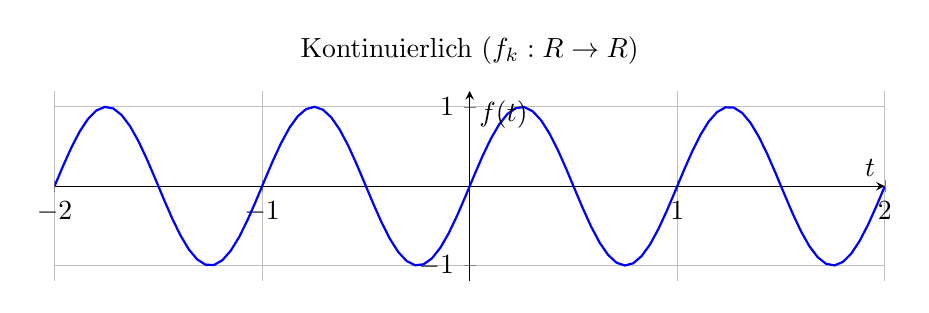
\begin{tikzpicture}
    \begin{axis}[
        width=\textwidth, % Nutzt die volle Breite der Minipage
        height=4cm,
        axis lines = middle,
        xlabel = $t$,
        ylabel = {$f(t)$},
        domain = -2:2,
        samples = 100,
        grid = major,
        trig format plots=rad,
        xtick={-4,-3,-2,-1,0,1,2,3,4},               % Hauptbeschriftung (ganze Zahlen)
        title={Kontinuierlich ($f_k: \mathbb{R} \rightarrow \mathbb{R}$)},
        ymin=-1.2, ymax=1.2 % Gleiche Skalierung wie rechts
    ]
        \addplot[blue, thick] {sin(x*2*pi)};
    \end{axis}
    \end{tikzpicture}
\end{center}
\begin{center}
    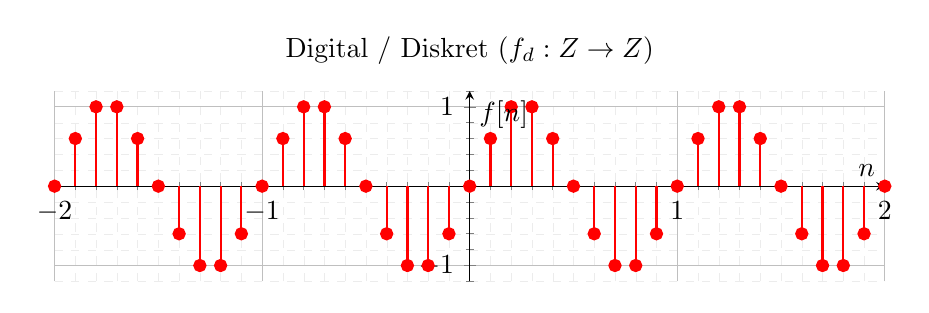
\begin{tikzpicture}
    \begin{axis}[
        width=\textwidth, % Nutzt die volle Breite der Minipage
        height=4cm,
        axis lines = middle,
        xlabel = $n$,
        ylabel = {$f[n]$},
        domain = -2:2,
        samples = 41, 
        trig format plots=rad,
        ytick={-3,-2,-1,0,1,2,3},          % Hauptbeschriftung (ganze Zahlen)
        minor y tick num=4,                % Erzeugt 9 Zwischenstufen -> Schritte von 0.1
        xtick={-4,-3,-2,-1,0,1,2,3,4},               % Hauptbeschriftung (ganze Zahlen)
        minor x tick num=9,                % Erzeugt 9 Zwischenstufen -> Schritte von 0.1
        grid = both,                       % Aktiviert Haupt- UND Nebengitter
        minor grid style={dashed=false, gray!15, ultra thin}, % Sehr feine, helle Linien für das 0.1-Raster
        title={Digital / Diskret ($f_d: \mathbb{Z} \rightarrow \mathbb{Z}$)},
        ymin=-1.2, ymax=1.2
    ]
        %%\addplot[gray, thin, ycomb, mark=*] {sin(x*2*pi)};
        \addplot[red, thick, ycomb, mark=*] {round(5*sin(x*2*pi))/5};
    \end{axis}
    \end{tikzpicture}
\end{center}

Meistens sind periodische Signale zwischen -1 und 1 wie zum Beispiel $f_k$ bzw $f_d$ 
interessant.
Eine wichtige Kenngröße von periodischen Signalen ist die Frequenz. 
Das ist die Anzahl der Wiederholungen pro Einheit (in diesem Fall Sekunden).
Sie wird in Hertz (Hz) angegeben. $f_k$ und $f_d$ haben eine Frequenz von 1 Hz.
Die Amplitude ist die maximale Auslenkung des Signals. $f_k$ und $f_d$ haben 
eine Amplitude von 1 und $0.5*sin(x)$ hat eine Amplitude von 0.5.

Zwei wichtige Kenngröße von digitalen Signalen sind die Abtastrate
und die Auflösung.

Die \textbf{Abtastrate} ist ein Maß für die Feinheit der Unterteilung der X-Achse
bzw. der Zeit. Sie wird ebenfalls in Hertz gemessen. Nehmen wir an, dass
das Signal $f_d$ in Sekunden angegeben ist, so ist seine Abtastrate 10Hz.

% TODO bessert machen
% \begin{center}
%     \begin{tikzpicture}
%     \begin{axis}[
%         width=\textwidth/2, % Nutzt die volle Breite der Minipage
%         height=4cm,
%         axis lines = middle,
%         xlabel = $n$,
%         ylabel = {$f_d[n]$},
%         domain = 0:10,
%         samples = 11, 
%         trig format plots=rad,
%         ytick={-3,-2,-1,0,1,2,3},          % Hauptbeschriftung (ganze Zahlen)
%         minor y tick num=4,                % Erzeugt 9 Zwischenstufen -> Schritte von 0.1
%         xtick={0,1,2,3,4,5,6,7,8,9},               % Hauptbeschriftung (ganze Zahlen)
%         xticklabels={1,2,3,4,5,6,7,8,9,10},
%         grid = both,                       % Aktiviert Haupt- UND Nebengitter
%         minor grid style={dashed=false, gray!15, ultra thin}, % Sehr feine, helle Linien für das 0.1-Raster
%         title={Digital / Diskret ($f_d: \mathbb{Z} \rightarrow \mathbb{Z}$)},
%         xmin=-0.5, xmax=9.5, ymin=-1.2, ymax=1.2,
%         xticklabel style={
%             yshift=-1.2cm % Schiebt die Zahlen 1 bis 11 unter den Graphen
%         },
%         xlabel style={
%             at={(ticklabel* cs:1)}, anchor=west % Setzt das "n" sauber ans Ende der Achse
%         },
%         ylabel style={
%             at={(ticklabel* cs:1)}, anchor=south % Setzt das "n" sauber ans Ende der Achse
%         }
%     ]
%         %%\addplot[gray, thin, ycomb, mark=*] {sin(x*2*pi)};
%         \addplot[red, thick, ycomb, mark=*] {round(5*sin((1/10)*x*2*pi))/5};
%     \end{axis}
%     \end{tikzpicture}
% \end{center}

Für die \textbf{Auflösung} muss ein maximaler und ein minimaler Wert festgelegt werden.
Dann ist die Auflösung die Anzahl der möglichen Werte zwischen dem
Maximalwert und dem Minimalwert. Für $f_d$ mit Minimalwert -1 und Maximalwert 1
wäre das 11.

Jedes stückweise stetige periodische Signal $S$ lässt sich, mithilfe der Fouriereihe,
als Summe von Sinus- und Cosinuskurven mit verschiedenen Frequenzen schreiben
\cite[2.2.1]{grueningen2008dsv}

Sei ein Signal $f_{max}$ die höchste dieser Frequenzen.
Das \textbf{Abtasttheorem} \cite{grueningen2008dsv} besagt, dass das
Signal $S$ wieder aus seiner Darstellung als digitales Signal $S_d$
rekonstruiert werden kann, wenn die Abtastrate von $S_d$ mindestens 
doppelt so groß ist wie $f_{max}$.

In der Signaltheorie beschreibt ein System etwas, das ein Signal $f(t)$ in ein
Signal $g(t)$ umwandelt. Ein digitales System schickt ein digitales Signal 
$f(n)$ auf ein anderes digitales Signal $g(n)$. Ein Beispiel ist das System,
das alle Werte eines Signals mit $0.5$ multipliziert.

\begin{figure}[ht]
    \centering
    \begin{tikzpicture}[
        system/.style={
            draw,
            rounded corners,
            minimum width=2.8cm,
            minimum height=1cm,
            align=center
        },
        arrow/.style={
            ->,
            >=stealth,
            thick
        }
    ]

        \node[] (f) {$f(t)$};
        \node[system, right=1cm of f] (Sys) {System};
        \node[right=1cm of Sys] (g) {$g(t)$};

        \draw[arrow] (f) -- (Sys);
        \draw[arrow] (Sys) -- (g);

    \end{tikzpicture}
    \caption{Darstellung eines Systems}
\end{figure}

\begin{figure}[ht]
    \centering
    \begin{tikzpicture}[
        system/.style={
            draw,
            rounded corners,
            minimum width=2.8cm,
            minimum height=1cm,
            align=center
        },
        arrow/.style={
            ->,
            >=stealth,
            thick
        }
    ]

        \node[] (f) {$sin(t)$};
        \node[system, right=1cm of f] (Sys) {*0.5};
        \node[right=1cm of Sys] (g) {$sin(t)*0.5$};

        \draw[arrow] (f) -- (Sys);
        \draw[arrow] (Sys) -- (g);

    \end{tikzpicture}
    \caption{Beispiel eines Systems}
\end{figure}

Weitere Eigenschaften von Systemen und Signalen sind in Grüningens Buch
digitale Signalverarbeitung \cite{grueningen2008dsv}.

\subsection{Darstellung  digitaler Audio}



Wie kann man einen Ton erzeugen? Ein Ton beschreibt eine
periodische Druckänderungen über die Zeit in der Luft. Solch eine
Druckänderung kann durch einen Lautsprecher erzeugt werden, in dem der
Lautsprecher analoges (kontinuierliches) elektrisches Signal erhält. Diese 
kann von einem DAC (Digital-zu-Analog-Konverter) erzeugt werden,
welcher wiederum ein digitales Signal erhält.

% erstellt mit chatGPT
\begin{figure}[ht]
    \centering
    \begin{tikzpicture}[
        signal/.style={
            draw,
            rounded corners,
            minimum width=2.8cm,
            minimum height=1cm,
            align=center
        },
        arrow/.style={
            ->,
            >=stealth,
            thick
        }
    ]

        \node[signal] (digital) {Digitales\\Signal};
        \node[signal, right=2.5cm of digital] (analog) {Analoges\\Signal};
        \node[signal, right=2.5cm of analog] (sound) {Ton};

        \draw[arrow] (digital) -- node[above] {DAC} (analog);
        \draw[arrow] (analog) -- node[above] {Lautsprecher} (sound);

    \end{tikzpicture}
    \caption{Vereinfachte Darstellung der Tonerzeugung}
    \label{fig:tonerzeugung}
\end{figure}

\subsubsection{Auflösung und Abtastrate}

Nun ist also die Frage, was für ein Signal der DAC erwartet. Da gibt es viele
verschiedene Möglichkeiten. Ein Standard für digitale Audio ist 
I2S (Inter-IC Sound). Das ist ein Protokoll, welches Stereoaudio, also 2 
Audiosignale, über 3 (manchmal 4) Leitungen überträgt.
\begin{enumerate}
    \item BCLK (Bit-Clock), manchmal auch Serial clock genannt, ist der Taktgeber.
    \item LRCLK (Left-Right-Clock), manchmal auch Word select genannt, gibt an, ob gerade Links oder Rechts übertragen
     wird.
    \item DIN/DOUT (Data in/Data out), manchmal auch Serial data genannt, überträgt die Audiodaten.
\end{enumerate}

\begin{figure}[h]
    \centering
    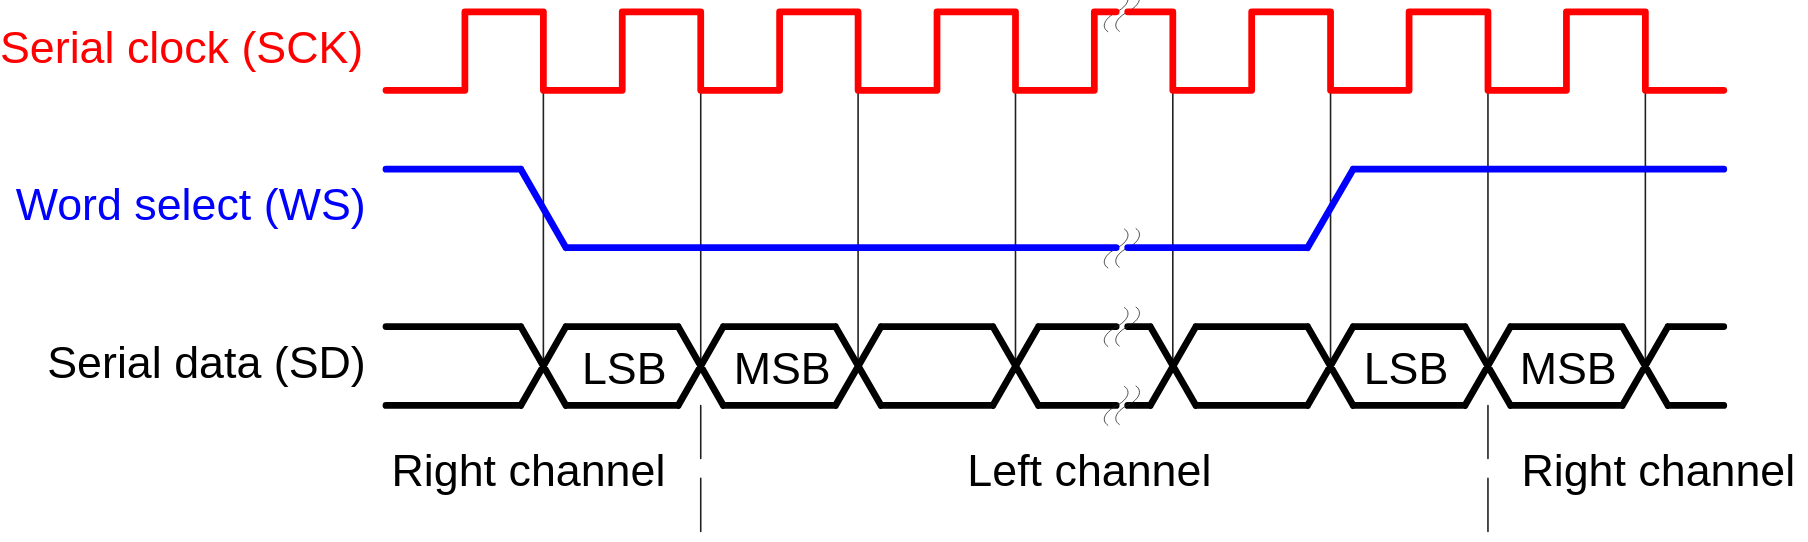
\includegraphics[width=0.9\textwidth]{fig/I2S.png}
    \caption{Zeitlicher Ablauf der I2S-Kommunikation,
    nach \cite{wdwd2011}.}
    \label{fig:I2S-leitungen}
\end{figure}



PCM-Daten \cite{jita2023} sind ein unkomprimiertes 
Audioformat bei dem Werte durch 8, 16, 24 oder 32 Bit unsigned Integern
dargestellt werden. Somit ist die Auflösung 8, 16, 24 oder 32 Bit.


Das menschliche Gehör kann in der Regel Frequenzen zwischen 20 und 20.000
Hertz wahrnehmen \cite{purves2001neuroscience}. 
Aus dem Abtasttheorem folgt, dass eine Abtastrate von
mindestens 40.000 Hz nötig ist, um Töne digital darzustellen.
Deshalb wurde 44100 als Abtastrate für CDs und 
infolge dessen auch für viele andere digitale Systeme gewählt. 
Hochwertige Systeme verwenden auch bis zu über 100 kHz.

